\documentclass{beamer}
\setbeamertemplate{footline}[page number]
\date{}
\author{}
\institute{}

%%%%%%% Put these names back in the final version 
%\\Aswathy Rajendra Kurup\\Meenu Ajith}
%\institute{Department of Electrical and Computer Engineering\\The University of New Mexico}
\setbeamercovered{transparent}
\usepackage{setspace}
\usepackage{array}
\usepackage[T1]{fontenc}
\usepackage{graphicx}
\usepackage{amsmath}
\usepackage{amsfonts}
\usepackage{amssymb}
\usepackage{makeidx}
\usefonttheme{serif}
\usepackage{multirow}
\usepackage{booktabs} 
\usepackage{rotating}
\usepackage{color}
\usepackage{float}
\usepackage[latin1]{inputenc}
\usepackage[english]{babel}
\usepackage{amsmath}
\usepackage{amsfonts}
\usepackage{eurosym}
\usepackage{rotating}
\usepackage{multicol}
\usepackage{pythonhighlight}
\usepackage[normalem]{ulem}
\newcommand{\ba}{{\bf a}}
\newcommand{\bb}{{\bf b}}
\newcommand{\bc}{{\bf c}}
\newcommand{\bd}{{\bf d}}
\newcommand{\be}{{\bf e}}
\newcommand{\bbf}{{\bf f}}
\newcommand{\bg}{{\bf g}}
\newcommand{\bh}{{\bf h}}
\newcommand{\bi}{{\bf i}}
\newcommand{\bk}{{\bf k}}
\newcommand{\bl}{{\bf l}}
\newcommand{\bm}{{\bf m}}
\newcommand{\bn}{{\bf n}}
\newcommand{\bo}{{\bf o}}
\newcommand{\bp}{{\bf p}}
\newcommand{\bq}{{\bf q}}
\newcommand{\br}{{\bf r}}
\newcommand{\bs}{{\bf s}}
\newcommand{\bt}{{\bf t}}
\newcommand{\bu}{{\bf u}}
\newcommand{\bv}{{\bf v}}
\newcommand{\bw}{{\bf w}}
\newcommand{\bx}{{\bf x}}
\newcommand{\by}{{\bf y}}
\newcommand{\bz}{{\bf z}}

\newcommand{\bA}{{\bf A}}
\newcommand{\bB}{{\bf B}}
\newcommand{\bC}{{\bf C}}
\newcommand{\bE}{{\bf E}}
\newcommand{\bG}{{\bf G}}
\newcommand{\bH}{{\bf H}}
\newcommand{\bI}{{\bf I}}
\newcommand{\bK}{{\bf K}}
\newcommand{\bL}{{\bf L}}
\newcommand{\bM}{{\bf M}}
\newcommand{\bO}{{\bf O}}
\newcommand{\bQ}{{\bf Q}}
\newcommand{\bR}{{\bf R}}
\newcommand{\bS}{{\bf S}}
\newcommand{\bT}{{\bf T}}
\newcommand{\bV}{{\bf V}}
\newcommand{\bW}{{\bf W}}
\newcommand{\bX}{{\bf X}}
\newcommand{\bY}{{\bf Y}}
\newcommand{\bZ}{{\bf Z}}
\newcommand\uptocnt{\stackrel{\mathclap{\normalfont\mbox{c}}}{\propto}}
\newcommand{\bpt}{{\bf pt}}
\newcommand{\bpl}{{\bf pl}}
\newcommand{\bdp}{{\bf dp}}
\newcommand{\btemp}{{\bf temp}}

\newcommand{\bmu}{{\boldsymbol \mu}}
\newcommand{\bSigma}{{\boldsymbol \Sigma}}
\newcommand{\bsigma}{{\boldsymbol \sigma}}
\newcommand{\bvarPhi}{{\boldsymbol \varPhi}}
\newcommand{\bvarphi}{{\boldsymbol \varphi}}
\newcommand{\bPhi}{{\boldsymbol \Phi}}
\newcommand{\bdelta}{{\boldsymbol \delta}}
\newcommand{\bZero}{{\bf 0}}
\newcommand{\bOne}{{\bf 1}}
\newcommand{\balpha}{{\boldsymbol \alpha}}
\newcommand{\bAlpha}{{\boldsymbol A}}
\newcommand{\btheta}{{\boldsymbol \theta}}

\newcommand{\softmax}{\text{softmax}}
\newcommand{\diag}{\text{diag}}
\newcommand{\sinc}{\mathrm{sinc}}
\newcommand{\argmin}{\mathop{\mathrm{argmin}}}
\newcommand{\infl}{\eta}
\newcommand{\Ind}{\mathrm{I}}
\newcommand{\Real}{\mathbb R}
\newcommand{\Intg}{\mathbb Z}
\newcommand{\Complex}{\mathbb C}
\newcommand{\Natural}{\mathbb N}
\newcommand{\Fourier}[1]{\mathcal{F} \{#1\}}
%\newcommand{\ii}{\mathbbm{i}}
\newcommand{\bphi}{\boldsymbol{\mathit{\phi}}}

\newcommand{\hs}{\hspace{2pt}}
\newcommand{\sign}{\text{sign}}
\author{Manel Mart\'inez-Ram\'on\\Meenu Ajith\\Aswathy Rajendra Kurup}

\usetheme{Madrid}
\usecolortheme{beaver}
\usepackage{tikz}
\usetikzlibrary{fit,arrows,calc,positioning}
\usepackage{listings}
\usepackage{xcolor}
\usepackage{emerald} 
\usepackage[T1]{fontenc} 
\usepackage{verbatim}
\usepackage{graphicx}
\usepackage{epsfig}
\usepackage{psfrag}
\usepackage[english]{babel}
\usepackage{listings}
\usepackage{courier}
\usepackage{color}
 \usepackage{vwcol} 
 \usepackage[english]{babel} % To obtain English text with the blindtext package
\usepackage{blindtext}
\definecolor{codegreen}{rgb}{0,0.6,0}
\definecolor{codegray}{rgb}{0.5,0.5,0.5}
\definecolor{codepurple}{rgb}{0.58,0,0.82}
\definecolor{backcolour}{rgb}{0.95,0.95,0.92}

\lstdefinestyle{mystyle}{
  backgroundcolor=\color{backcolour},   commentstyle=\color{codegreen},
  keywordstyle=\color{magenta},
  numberstyle=\tiny\color{codegray},
  stringstyle=\color{codepurple},
  basicstyle=\ttfamily\footnotesize,
  breakatwhitespace=false,         
  breaklines=true,                 
  captionpos=b,                    
  keepspaces=true,                 
  numbers=left,                    
  numbersep=5pt,                  
  showspaces=false,                
  showstringspaces=false,
  showtabs=false,                  
  tabsize=2
}
\lstset{style=mystyle}

%% Stuff for movies

% %\newcommand{\bt}{{\bf t}}
% \newcommand{\br}{{\bf r}}
% \newcommand{\bs}{{\bf s}}
% \newcommand{\by}{{\bf y}}
% \newcommand{\bz}{{\bf z}}
% \newcommand{\bx}{{\bf x}}
% \newcommand{\bw}{{\bf w}}
% \newcommand{\be}{{\bf e}}
% \newcommand{\bbf}{{\bf f}}
% \newcommand{\bb}{{\bf b}}
% \newcommand{\bd}{{\bf d}}
% \newcommand{\bA}{{\bf A}}
% \newcommand{\bB}{{\bf B}}
% \newcommand{\bL}{{\bf L}}
% \newcommand{\bM}{{\bf M}}

% \newcommand{\bC}{{\bf C}}
% \newcommand{\bI}{{\bf I}}
% \newcommand{\bK}{{\bf K}}
% \newcommand{\bk}{{\bf k}}
% \newcommand{\bT}{{\bf T}}
% \newcommand{\bV}{{\bf V}}
% \newcommand{\bW}{{\bf W}}
% \newcommand{\bX}{{\bf X}}
% \newcommand{\bY}{{\bf Y}}
% \newcommand{\bZ}{{\bf Z}}
% \newcommand{\bm}{{\bf m}}
% \newcommand{\bpt}{{\bf pt}}
% \newcommand{\bpl}{{\bf pl}}
% \newcommand{\bdp}{{\bf dp}}
% \newcommand{\btemp}{{\bf temp}}
% \newcommand{\bl}{{\bf l}}
% \newcommand{\bu}{{\bf u}}
% \newcommand{\bmu}{{\boldsymbol \mu}}
% \newcommand{\bSigma}{{\boldsymbol \Sigma}}
% \newcommand{\bLambda}{{\boldsymbol \Lambda}}

% \newcommand{\bsigma}{{\boldsymbol \sigma}}
% \newcommand{\bvarphi}{{\boldsymbol \varPhi}}
% \newcommand{\btheta}{{\boldsymbol \theta}}
% \newcommand{\bZero}{{\bf 0}}
% \newcommand{\balpha}{{\boldsymbol \alpha}}
% \newcommand{\bpi}{{\boldsymbol \pi}}
% \newcommand{\bxi}{{\boldsymbol \xi}}
% \newcommand{\bdelta}{{\boldsymbol \delta}}
\lstset{
	language=Python,
	basicstyle=\footnotesize\ttfamily\color{black},
	commentstyle = \footnotesize\ttfamily\color{red},
	keywordstyle=\footnotesize\ttfamily\color{blue},
	stringstyle=\footnotesize\ttfamily\color{black},
%	columns=fixed,
%	numbers=left,    
	numberstyle=\tiny,
	stepnumber=1,
	numbersep=5pt,
	tabsize=1,
	extendedchars=true,
	breaklines=true,            
	frame=b,         
	showspaces=false,
	showtabs=true,
	xleftmargin=6pt,
	framexleftmargin=6pt,
	framexrightmargin=2pt,
	framexbottommargin=4pt,
	showstringspaces=false      
}

\lstloadlanguages{
         Python
}

%\graphicspath{ {./images/} }  % Figures path - used in graphicx

%\selectcolormodel{cmyk}

\mode<presentation>

\newcommand{\dred}{darkred!90!black}
\newcommand{\written}{\ECFJD\textcolor{cyan!50!white}}
\newcommand{\hlight}{\textcolor{\dred}}
\newcommand{\Ex}{\textcolor{\dred}{Ex. }}

% remove navigation symbols in full screen mode
\setbeamertemplate{navigation symbols}{}  
\setbeamertemplate{blocks}[rounded][shadow=false]
\setbeamercolor{note page}{fg=black}

\setbeamercolor{title}{fg=\dred}
\setbeamercolor{frametitle}{fg=white}
\setbeamercolor{frametitle}{bg=\dred}
\setbeamercolor{structure}{fg=black,bg=white}
\setbeamercolor{background canvas}{bg=white,fg=black}
\setbeamercolor{normal text}{fg=black,bg=white}
\setbeamercolor{item}{fg=red!80!black,bg=white!}
\addtobeamertemplate{block begin}{\setbeamercolor{block title}{fg=white,bg=\dred}
\setbeamercolor{block body}{fg=white,bg=gray}}{}


\title{6. Attention-based networks}
\subtitle{6.4. Large-scale pretraining with transformers}

\addtobeamertemplate{frametitle}{}


\begin{document}
\maketitle


\begin{frame}{Introduction}
\begin{itemize}
\item In the previous lessons we have seen models trained for specific tasks (English to French translation, image classification).
\item Pretraining models are becoming common for better generalized models and generalist models. 
\item Transformers for machine translation consist of an encoder for the representation of input sequences and one for generating target sequences.
\item In general, transformers can be used as encoder-decoder, encoder only, and decoder only. 
\end{itemize}
\end{frame}
\begin{frame}{Encoder-only structures}
\begin{itemize}
    \item Remember the self-attention mechanisms that given a sequence $\bx_1, \cdots, \bx_N$ outputs a sequence $\by_1, \cdots, \by_n$ with the same shape, where 
    \begin{equation}
        \by_n = \sum_{i=1}^N \alpha(\bx_i,\bx_n)\bx_n = \balpha_n^\top \bx_n
    \end{equation}
    \item In additive attention we have 
    \begin{equation}
    \begin{split}
        a(\bx_i,\bx_n) & = \bw_f \tanh(\bW_q\bx_n+\bW_k \bx_i)\\
        \balpha_n & = \softmax\left( a(\bx_1,\bx_n), \cdots, a(\bx_N,\bx_n) \right)
    \end{split}
    \end{equation}
\item Therefore, for a sequence of $N$ elements, a self attention mechanism produces a matrix $\left[\balpha_1, \cdots, \balpha_N\right] \in \mathbb{R}^{N\times N}$ of self attention scores.  
\end{itemize}
\end{frame}
\begin{frame}{Encoder-only structures}
    \begin{itemize}
        \item A multi-head attention mechanism with $M$ heads produces an array of dimensions $N\times N \times M$ attention scores, which are used to construct $M$ representations $\bh_{n,m}$ of each element $\bx_n$. 
        \item Each representation is then linearly combined with a transformation matrix as 
        \begin{equation}
            \by_n = \bW^\top \bh_n
        \end{equation}
where $\bh_n$ is the concatenation of vectors $\bh_{n,m}$.        
       
    \end{itemize}
\end{frame}
\begin{frame}{Encoder-only structures}
\begin{itemize}
    \item An encoder only is a set of self-attention layers with a fully connected layer that produces a classification. 
\end{itemize}
\begin{center}
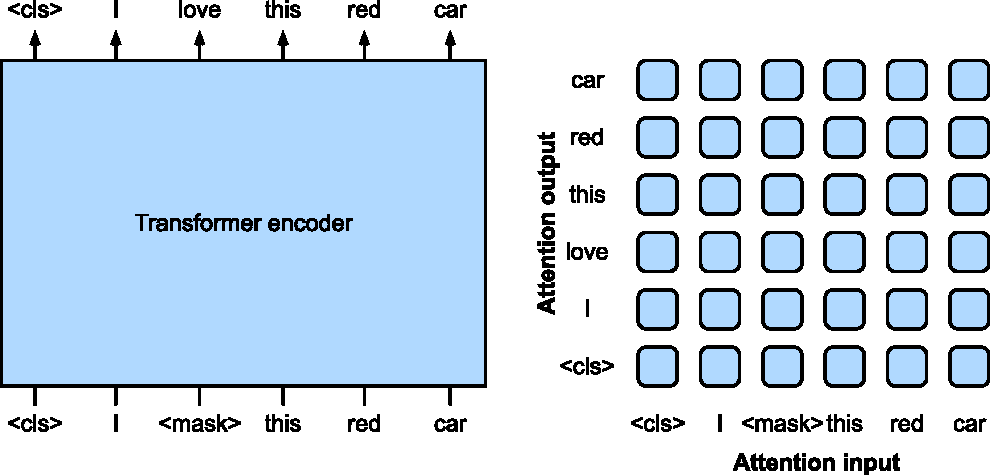
\includegraphics[scale=0.5]{Module 6 (Attention-based networks)/pics/bert-encoder-only.pdf}
\end{center}
\begin{itemize}
    \item This is the pre-trained bidirectional Encoder Representation from transformers (BERT). 
\end{itemize}
\end{frame}

\begin{frame}{Encoder-only structures}{Pretraining BERT}
\begin{itemize}
    \item A BERT is pre-trained by using masked sequences as inputs and using the unmasked sequences as outputs, with the <cls> token included. 
    \item A cross-entropy is used as a criterion. 
    \item It is called bidirectional because the predicted word depends on the previous and posterior tokens. 
    \item This training is unsupervised, as sequences do not have labels. Therefore, large databases (as Wikipedia) can be ``easily'' used.
    \item The output token corresponding to the input <cls> is then used to produce a classification after a fine-tuning. 
\end{itemize}    
\end{frame}

\begin{frame}{Encoder-only structures}{Fine tuning BERT}
\begin{itemize}
\item The <cls> output is then a global representation of the sequence. 
    \item The BERT can be fine-tuned to perform specific tasks.
\end{itemize}
    \begin{center}
        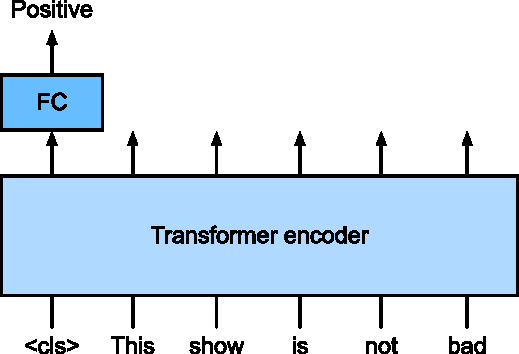
\includegraphics[scale=0.5]{Module 6 (Attention-based networks)/pics/bert-finetune-classification.pdf}
    \end{center}
\begin{itemize}
    \item Fully connected layers can be connected to the <cls> to train the whole structure to perform, for example, a sentiment analysis task.
    
\end{itemize}
\end{frame}
\begin{frame}{Encoder-only structures}{Fine tuning BERT}
\begin{itemize}
\item Cross entropy and backpropagation is used to train the fully connected layers from scratch while the BERT structure is just updated.  

    \item Based on this idea, and using a 350M parameter structure trained with 250 Billion tokens, BERT has been used for representation spans of text, computer vision, and others. 
\end{itemize}
\end{frame}

\begin{frame}{Encoder-decoder structures}
    \begin{itemize}
        \item The encoder-only structure cannot predict text for tasks as machine translation because the output sequence has the same length as the input. 
        \item The encoder-decoder for machine translation first produces a representation of length N. 
        \item The decoder produces a matrix of $N\times m$ attention scores (or equivalently, multi-head scores) to predict the next token. 
        \item This is called cross-attention.  
    \end{itemize}
\end{frame}

\begin{frame}{Encoder-decoder structures}
    \begin{itemize}
    \item BART and T5 are two encoder-decoder schemes that are pre-trained with large text corpora. 
    \item Both reconstruct text during the pre-training. BART uses deletion, permutation, and rotation besides masking. 
    \end{itemize}
\end{frame}

\begin{frame}{Encoder-decoder structures}{Pretraining T5}
\vspace{-0.6cm}
\begin{itemize}
    \item The Text-to-Text Transfer Transformer (T5) is trained to predict consecutive spans with special tokens. 
\end{itemize}   
\begin{center}
    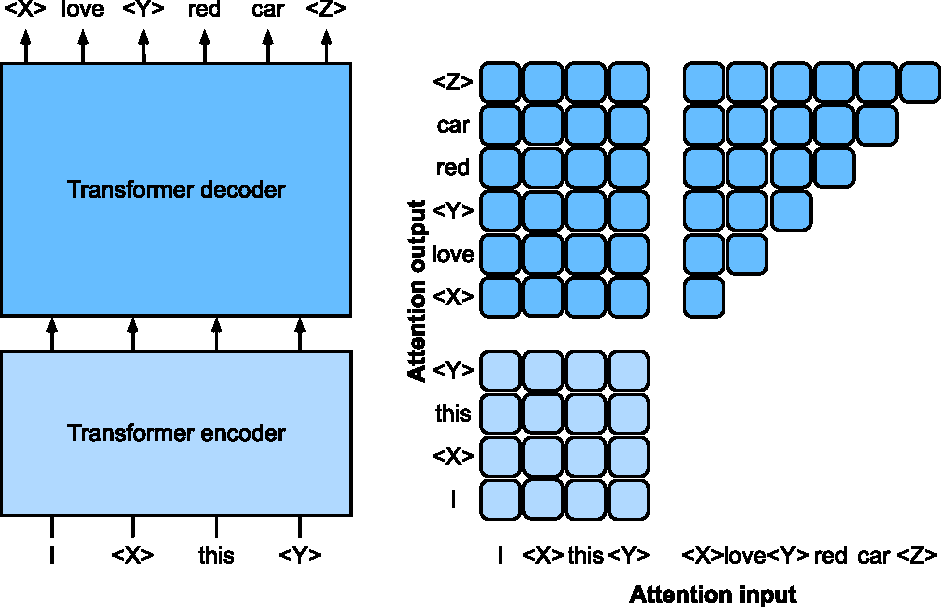
\includegraphics[scale=0.5]{Module 6 (Attention-based networks)/pics/t5-encoder-decoder.pdf}
\end{center}
\begin{itemize}
    \item The decoder self-attention is causal (it attends only to past tokens.) 
\end{itemize} 
\end{frame}
\begin{frame}{Encoder-decoder structures}{Fine-tuning T5}
\begin{itemize}
    \item T5 can be fine-tuned to perform various specific tasks in the same text-to-text problem.
    \begin{itemize}
        \item T5 includes the task description at the input. 
        \item T5 can produce sequences with arbitrary lengths. 
        \item No additional layers are required. 
    \end{itemize}
    \begin{center}
        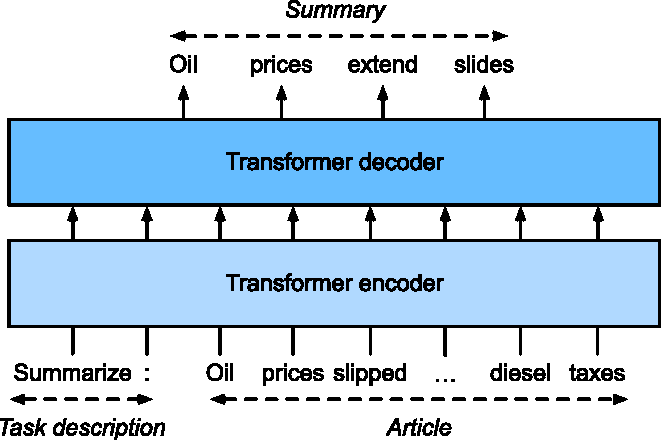
\includegraphics[scale=0.5]{Module 6 (Attention-based networks)/pics/t5-finetune-summarization.pdf}
    \end{center}
\end{itemize}    
\end{frame}
\begin{frame}{Encoder-decoder structures}{Fine-tuning T5}
    \begin{itemize}
        \item The 11-billion-parameter T5 (T5-11B) achieved state-of-the-art results on multiple encoding (e.g., classification) and generation (e.g., summarization) benchmarks. 
        \item  The Imagen structure, text is input to a frozen 4.6 Billon parameter T5 encoder (T5-XXL) to produce images.
    \end{itemize}
    \begin{center}
        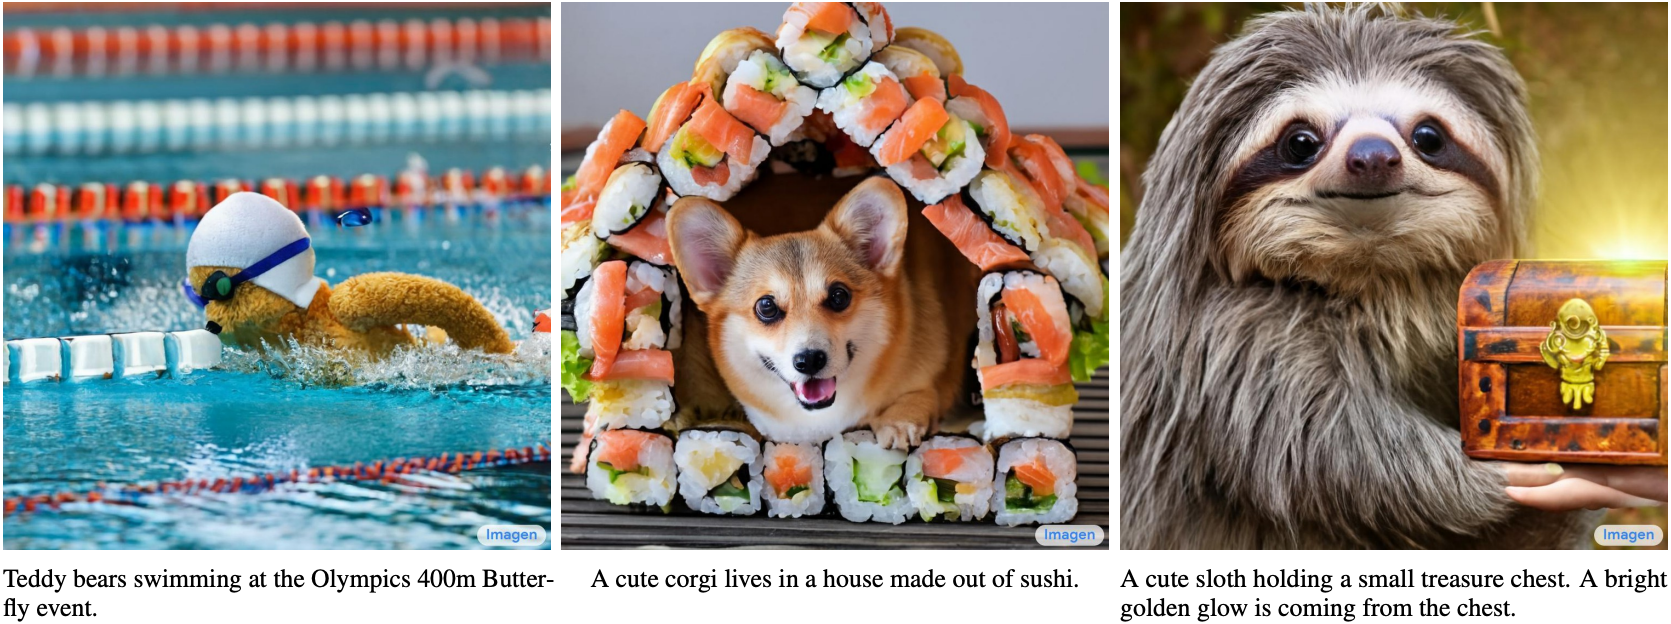
\includegraphics[scale=0.2]{Module 6 (Attention-based networks)/pics/imagen.png}
    \end{center}
\end{frame}

\begin{frame}{Decoder-only structures}{GPT and GPT-2}
\begin{itemize}
    \item The decoder-only structures remove the encoder and the encoder-decoder cross attention. 
    \item This allows to train large models with any text databases. 
    \item The Generative Pre-Training model is based on a decoder. 
\end{itemize}    
\begin{center}
    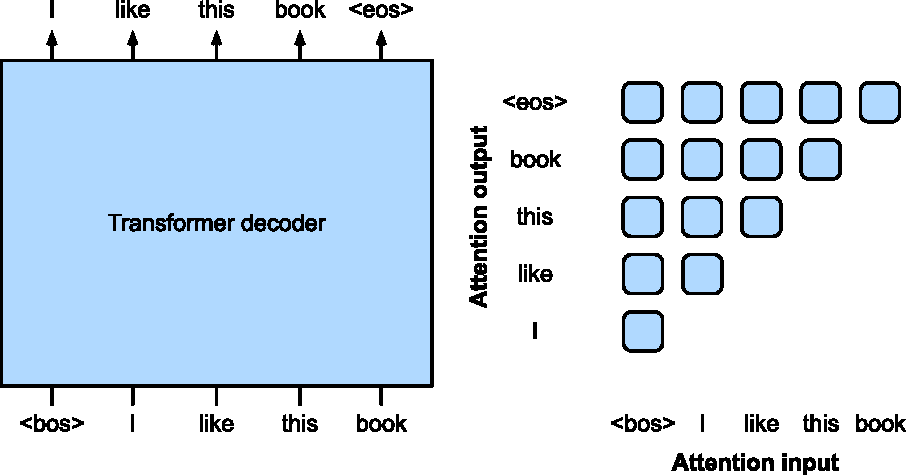
\includegraphics[scale=0.4]{Module 6 (Attention-based networks)/pics/gpt-decoder-only.pdf}
\end{center}
\begin{itemize}
    \item The GPT is trained with the output as the input sequence shifted.
\end{itemize}
\end{frame}
\begin{frame}{Decoder-only structures}{GPT and GPT-2}
    \begin{itemize}
        \item GPT (2018) has 100 million parameters and needs to be fine-tuned for individual downstream tasks. 
        \item GPT-2 (2019) uses pre-normalization  and improved initialization and weight-scaling 
        \item GPT-2 was pre-trained on 40 GB of text and had 1.5 billion parameters.
        \item GPT-2 obtained state-of-the-art results on language modeling benchmarks and promising results on multiple other tasks without updating the parameters or architecture.
    \end{itemize}
\end{frame}
\begin{frame}{GPT3}
\begin{center}
    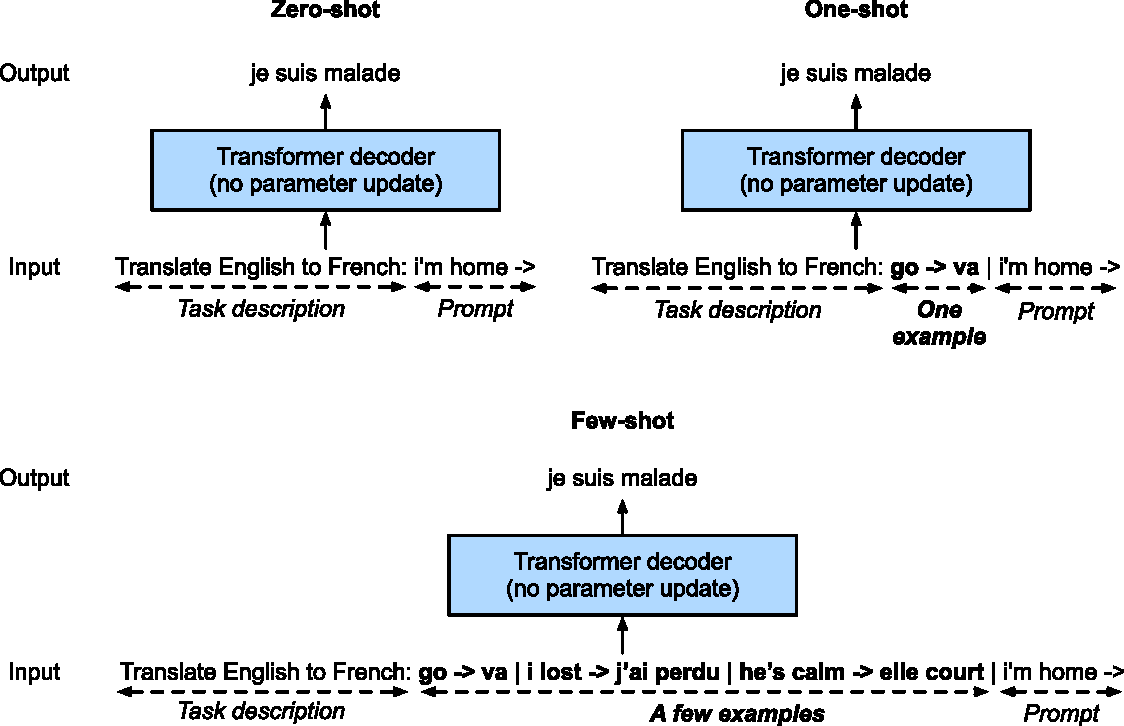
\includegraphics[scale=0.5]{Module 6 (Attention-based networks)/pics/gpt-3-xshot.pdf}
\end{center}    
\end{frame}
\end{document}